\documentclass[english]{sigplanconf}
\usepackage[T1]{fontenc}
\usepackage[latin9]{inputenc}
\usepackage[english]{babel}
\usepackage{verbatim}
\usepackage{refstyle}
\usepackage{float}
\usepackage{textcomp}
\usepackage{amsthm}
\usepackage{amstext}
\usepackage{amsmath}
\usepackage{amssymb}
\usepackage{graphicx}
\usepackage{xcolor}
\usepackage[lined,linesnumbered,commentsnumbered]{algorithm2e}
\theoremstyle{definition}
\newtheorem{example}{Example}[section]
\newtheorem*{notation}{Notation}

% ============================================================
%% Uncomment the next few lines to get sf url links:
%\usepackage{url}            
%\makeatletter
%\def\url@leostyle{%
%  \@ifundefined{selectfont}{\def\UrlFont{\sf}}{\def\UrlFont{\small\sffamily}}}
%\makeatother
%\urlstyle{leo} % Now actually use the newly defined style.
%% Choose coloured or b/w links:
\usepackage[pdftex,colorlinks=true,pdfstartview=FitV,
 linkcolor=black,citecolor=black,urlcolor=black]{hyperref}
% \usepackage{hyperref}
\usepackage{needspace}
\newcommand{\needlines}[1]{\Needspace{#1\baselineskip}}
% ============================================================
% Markup macros for proof-reading
\usepackage{ifthen}
\usepackage[normalem]{ulem} % for \sout
\usepackage{xcolor}
\newcommand{\ra}{$\rightarrow$}
\newboolean{showedits}
\setboolean{showedits}{true} % toggle to show or hide edits
\ifthenelse{\boolean{showedits}}
{
	\newcommand{\ugh}[1]{\textcolor{red}{\uwave{#1}}} % please rephrase
	\newcommand{\ins}[1]{\textcolor{blue}{\uline{#1}}} % please insert
	\newcommand{\del}[1]{\textcolor{red}{\sout{#1}}} % please delete
	\newcommand{\chg}[2]{\textcolor{red}{\sout{#1}}{\ra}\textcolor{blue}{\uline{#2}}} % please change
}{
	\newcommand{\ugh}[1]{#1} % please rephrase
	\newcommand{\ins}[1]{#1} % please insert
	\newcommand{\del}[1]{} % please delete
	\newcommand{\chg}[2]{#2}
}
% ============================================================
% Put edit comments in a really ugly standout display
%\usepackage{ifthen}
\usepackage{amssymb}
\newboolean{showcomments}
\setboolean{showcomments}{true}
%\setboolean{showcomments}{false}
\newcommand{\id}[1]{$-$Id: scgPaper.tex 32478 2010-04-29 09:11:32Z oscar $-$}
\newcommand{\yellowbox}[1]{\fcolorbox{gray}{yellow}{\bfseries\sffamily\scriptsize#1}}
\newcommand{\triangles}[1]{{\sf\small$\blacktriangleright$\textit{#1}$\blacktriangleleft$}}
\ifthenelse{\boolean{showcomments}}
%{\newcommand{\nb}[2]{{\yellowbox{#1}\triangles{#2}}}
{\newcommand{\nbc}[3]{
 {\colorbox{#3}{\bfseries\sffamily\scriptsize\textcolor{white}{#1}}}
 {\textcolor{#3}{\sf\small$\blacktriangleright$\textit{#2}$\blacktriangleleft$}}}
 \newcommand{\version}{\emph{\scriptsize\id}}}
{\newcommand{\nbc}[3]{}
 \renewcommand{\ugh}[1]{#1} % please rephrase
 \renewcommand{\ins}[1]{#1} % please insert
 \renewcommand{\del}[1]{} % please delete
 \renewcommand{\chg}[2]{#2} % please change
 \newcommand{\version}{}}
\newcommand{\nb}[2]{\nbc{#1}{#2}{orange}}
\newcommand{\here}{\yellowbox{$\Rightarrow$ CONTINUE HERE $\Leftarrow$}}
\newcommand\rev[2]{\nb{TODO (rev #1)}{#2}} % reviewer comments
\newcommand\fix[1]{\nb{FIX}{#1}}
\newcommand\todo[1]{\nb{TO DO}{#1}}
\newcommand\on[1]{\nbc{ON}{#1}{red}} % add more author macros here
\newcommand\ml[1]{\nbc{ML}{#1}{violet}} % add more author macros here
%\newcommand\XXX[1]{\nbc{XXX}{#1}{blue}}
%\newcommand\XXX[1]{\nbc{XXX}{#1}{brown}}
%\newcommand\XXX[1]{\nbc{XXX}{#1}{cyan}}
%\newcommand\XXX[1]{\nbc{XXX}{#1}{darkgray}}
%\newcommand\XXX[1]{\nbc{XXX}{#1}{gray}}
%\newcommand\XXX[1]{\nbc{XXX}{#1}{magenta}}
%\newcommand\XXX[1]{\nbc{XXX}{#1}{olive}}
%\newcommand\XXX[1]{\nbc{XXX}{#1}{orange}}
%\newcommand\XXX[1]{\nbc{XXX}{#1}{purple}}
%\newcommand\XXX[1]{\nbc{XXX}{#1}{red}}
%\newcommand\XXX[1]{\nbc{XXX}{#1}{teal}}
%\newcommand\XXX[1]{\nbc{XXX}{#1}{violet}}
% ============================================================


% Alter some LaTeX defaults for better treatment of figures:
    % See p.105 of "TeX Unbound" for suggested values.
    % See pp. 199-200 of Lamport's "LaTeX" book for details.
    %   General parameters, for ALL pages:
    \renewcommand{\topfraction}{0.9}	% max fraction of floats at top
    \renewcommand{\bottomfraction}{0.8}	% max fraction of floats at bottom
    %   Parameters for TEXT pages (not float pages):
    \setcounter{topnumber}{2}
    \setcounter{bottomnumber}{2}
    \setcounter{totalnumber}{4}     % 2 may work better
    \setcounter{dbltopnumber}{2}    % for 2-column pages
    \renewcommand{\dbltopfraction}{0.9}	% fit big float above 2-col. text
    \renewcommand{\textfraction}{0.07}	% allow minimal text w. figs
    %   Parameters for FLOAT pages (not text pages):
    \renewcommand{\floatpagefraction}{0.7}	% require fuller float pages
	% N.B.: floatpagefraction MUST be less than topfraction !!
    \renewcommand{\dblfloatpagefraction}{0.7}	% require fuller float pages

	% remember to use [htp] or [htpb] for placement

\begin{document}
\special{papersize=8.5in,11in}
\setlength{\pdfpageheight}{\paperheight}
\setlength{\pdfpagewidth}{\paperwidth}

\conferenceinfo{CONF 'yy}{Month d--d, 20yy, City, ST, Country}
\copyrightyear{20yy} 
\copyrightdata{978-1-nnnn-nnnn-n/yy/mm} 
\doi{nnnnnnn.nnnnnnn}

\frenchspacing

\title{Efficient regular expressions that produce parse trees}

\authorinfo{Nobody}

\authorinfo{Nobody}
      
\authorinfo{Nobody}

\maketitle

\begin{abstract}
Regular expressions naturally and intuitively define parse trees that describe
the text that they're parsing.
But existing approaches fail to keep track of all regex matches within the parse trees.
We describe a technique for building
up the complete parse tree resulting from matching a text against
a regular expression.

In standard TDFA matching, all paths through the NFA are walked simultaneously,
as if in different threads, where inside each thread, it is fully
known when which capture group was entered or left. We extend this
model to keep track of not just the last opening and closing of capture
groups, but all of them. We do this by storing, in every thread, using
the fly-weight pattern, a history of the all groups. Thus, we log
enough information during parsing to build up the complete AST at
the end of parsing.
\end{abstract}


\section{Introduction}

\global\long\def\regex{\text{\text{regular expression}}}
A regular expression can easily describe that a text matches a comma
separated values file, but it is unable to extract all the values.
Instead it will only give a single instance of values: \texttt{((.*?),(\textbackslash d+);)+} might describe a dataset of ASCII names
with their numeric label. Matching the regular expression on \texttt{``Tom
Lehrer,1;Alan Turing,2;''} will confirm that the list is well formed,
but the match will only contain \texttt{``Tom Lehrer''} for the
second capture group and \texttt{``1''} for the third. That is,
the parse tree found by the \textsc{posix} is seen in \Figref{posix}.

\begin{figure}[h]
\centering
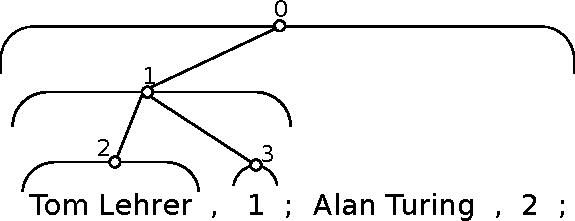
\includegraphics[width=.75\linewidth]{graphs/posix_parse}
\caption{\figlabel{lehrer-posix} Parse tree produced by \textsc{posix}-compatible matching \texttt{((.*?),(\textbackslash d+);)+} against input ``Tom
Lehrer,1;Alan Turing,2;''.}
\figlabel{posix}
\end{figure}

With our algorithm we are able to reconstruct the full parse
tree after the matching phase is done, as seen in \Figref{our-tree}.

\begin{figure}[h]
\centering
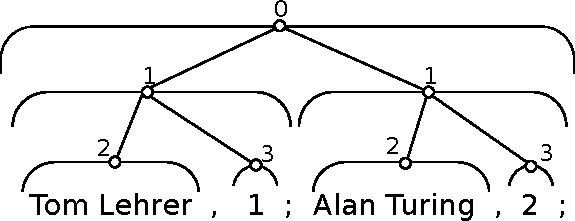
\includegraphics[width=.75\linewidth]{graphs/full_parse}
\caption{\figlabel{lehrer-tree} Parse tree produced by our approach matching regular expression \texttt{((.*?),(\textbackslash d+);)+} against input ``Tom
Lehrer,1;Alan Turing,2;''}
\figlabel{our-tree}
\end{figure}

The amortized run time of our approach is $O(m^2n)$, where $m$ is
the length of the regular expression and $n$ is the length of the
parsed string. It is, to the best of our knowledge, the first
algorithm to achieve this bound, while extracting parse trees. The
best-known algorithm to parse regular expressions, without extracting
parse trees, run in time $O(m n)$\cite{Sedg90a}.

\subsection{More powerful than standard regular expressions}
\seclabel{power}
It may at first seem as if all capture groups can always, equivalently,
be extracted by splitting the input, and then applying sub-regular
expressions on the splits.  This is, for example, an entirely valid
strategy to extract the parse tree in \Figref{lehrer-tree}.  However,
this can quickly become an exercise of writing an entire parser,
using no regular expression engine at all, even if the underlying
grammar is entirely regular.  The following grammar is hard to parse
using a regular expression engine, even though it is regular.

Consider a file of semicolon-terminated records, each record consisting
of a comma-separated pair of entries, and each entry can be escaped
to contain semicolons, as in the regular expression
\texttt{((".*?"|[a-z]*),(".*?"|[a-z]*);)+}. Here, expression
\texttt{.*?} is a non-greedy match which will be discussed in more
detail in \Secref{algo}.  This language contains, for example, the
string: ``"h;i",there;"h;,i",Paul;''.  It is easy to see that, in
order to extract all four capture group matches, it is insufficient
to split the input at the semicolon, as that would split the field
``h;i'' in half.  More involved examples, where hand-written parsers
become harder to make, are easily constructed.  In contrast, our
approach yields the entire parse tree, simply from the regular
expression.



\subsection{Motivation}

This is the age of big data, and the first step of processing big
data is often to parse strings. As an example, consider log files.
What makes data huge is typically repetition. As Jacobs\cite{Jaco09a}
noted, ``What makes most big data big is repeated observations over
time and/ or space,'' and thus log files grow large frequently. At
the same time, they provide important insight into the process that
they are logging, so their parsing and understanding is important. 

Regular expressions make for scalable and efficient lightweight parsers.\cite{Kart96a} 

The parsing abilities of regular expression have \chg{evoked}{provoked} Meiners to declare
that for intrusion detection, ``fast and scalable RE matching is
now a core network security issue.'' \cite{Mein10a}

For example, Arasu et al. \cite{Aras12a} demonstrate how regular
expressions are used in Bing to validate data, by checking whether
the names of digital cameras in their database are valid.

Parsers that can return abstract syntax trees are more useful than
ones that only give a flat list of matches. Of course only regular
grammars can be matched by our approach.

\section{Algorithm}
\seclabel{algo}

Let us recall what NFAs and DFAs are. A DFA is a state machine that
will walk over the transition graph, one step for every input
character. The choice of transition is limited by the transition's
character range. A transition can only be followed if the current
input character is inside transition's character range. NFAs differ
from DFAs in that for some input character and some state, there
may be more than one applicable transition. If there is, an
NFA will magically guess the correct one. \autoref{fig:example-automaton}
shows an example of an NFA's transition graph. For the moment, let
us discuss regular expression matching on NFAs. Assuming that the
NFA just magically knows the right transition lets us focus on the
important things, greediness control and capture groups.

Conceptually, our approach is the following pipeline of four stages.
\begin{enumerate}
  \item Parse the regular expression string into an AST.
  \item Transform the AST to an NFA.
  \item Transform the NFA to a DFA.
  \item Compactify the DFA.
\end{enumerate}

In reality, things are a little more involved, since the transformation
to DFA is lazy, and the compactification only happens after no lazy
compilation occurred in a while. Worse, compactification can be
undone if needed. We'll get back to these details in \secref{implementation}.
Let's discuss the stages in turn, starting with 2, since step 1,
the parsing of the regular expression grammar, is reasonably
straightforward.

\subsection{Thompson's construction} 

We transform the AST of the regular expression into an NFA,
in a modified version of Thompson's NFA construction. To
control greedines, or discern capture groups, our approach adds
$\varepsilon$ transitions to the transition graph. An
$\varepsilon$-transition has no input range assigned, and can thus always
be used. It does not consume an input character.
The additions are needed for greediness control and capture groups.
Let's look at both, in turn.

To see the importance of greediness control, consider again the regular
expression \texttt{((.*?),(\textbackslash{}d+);)+}. The question
mark sets the \texttt{.*} part of the regular expression to
\emph{non-greedy}, which means that it will match as little as
possible while still producing a valid match, if any.  Without
provisioning \texttt{.*} to be non-greedy, a matching against input
\texttt{``Tom Lehrer,1;Alan Turing,2;''} would match as much as
possible into the first capture group, including the record separator
`,'.  Thus, the first capture group would suddenly contain only one
entry, and it would contain more than just names, namely``Tom
Lehrer,1;Alan Turing''.  This is, of course, not what we expect.
Non-greediness, here, ensures that we get ``Tom Lehrer'', then
``Alan Turing'' as the matches of the first capture group.

\begin{figure}[h]
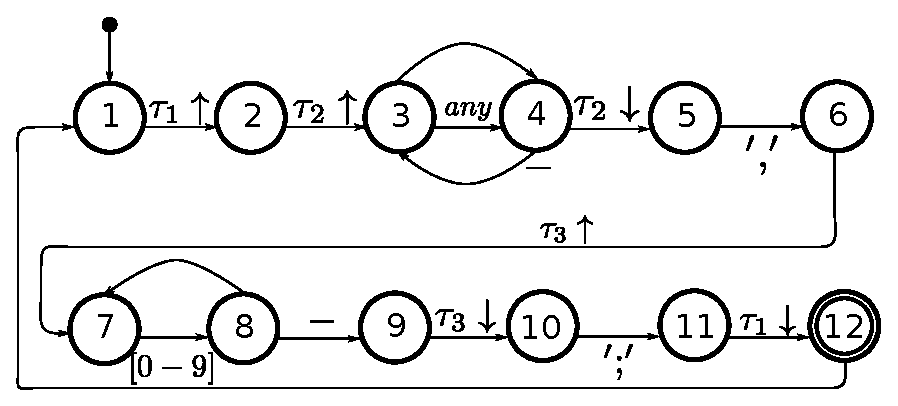
\includegraphics[width=\linewidth]{graphs/lehrer_automaton}

\caption{\label{fig:example-automaton}
Automaton for \texttt{((.*?),(\textbackslash{}d+);)+} 
In the diagram, ``$-$'' stands for low priority. $\tau_n\uparrow$ is the opening tag for capture group $n$, likewise, $\tau_1\downarrow$ is the closing tag for capture group $n$.}
\end{figure}


In the NFA, we model greedy repetition or non-greedy repetition of
an expression in two steps:

\begin{enumerate}
\item We construct an NFA graph for the expression, without any repetition.  
\autoref{fig:example-automaton} shows how this plays out in our running example, which contains the expression \texttt{.*?}. An automaton for \texttt{.} is constructed. The expression \texttt{.} is modeled as just two nodes labeled 3 and 4, and a transition labeled ``any''
between them.  

\item We add prioritized transitions to model repetition. In our example, repeating is achieved by adding two $\varepsilon$
transitions: one from 4 back to 3, to match more than one time any
character, and another one from 3 to 4, to enable matching nothing
at all.  Importantly, the transition from 4 back to 3 is marked as
low priority (the ``--'' sign) while the transition leaving the automaton, from 4
to 5, is unmarked, which means normal priority.  This means that
the NFA will prefer leaving the repeating expression, rather than
staying in it.  If the expression were greedy, then we would mark
the transition from 3 to 5 as low-priority, and the NFA would prefer
to match any character repeatedly. 

\end{enumerate}



More generally, the NFA will prefer to follow transitions of normal
priority over those of low priority. Rather than formalize this
notion of preference on NFAs, we come back to prioritized edges when
discussing the transformation from NFA states to DFA states.

\begin{figure*}[tb] 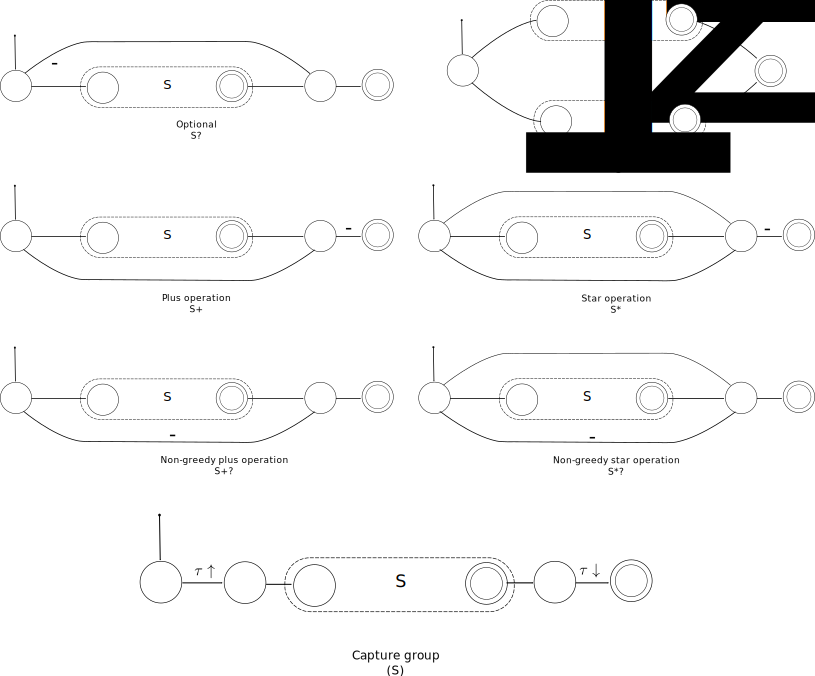
\includegraphics[width=\linewidth]{graphs/thompson}
\caption{Modified Thompson~\cite{Thom68a} construction of the
automaton: \ugh{Decent} \ins{Descend?} into the abstract syntax tree of the regular
expression and expand the constructs recursively.}
\label{fig:thompson-construction} 
\end{figure*}

To model capture groups in the NFA, we add \emph{commit tags} to the
transition graph. The transition into a capture group is tagged by a
commit, the transition to leave a capture group is tagged by a another
commit. We distinguish opening and closing commits. The NFA keeps a
history for every transition with a commit. Each time the transition
is walked, the current position \ins{in the input string} is added to its history. 

We model histories as a linked list, where the payload of each node
is a position.  Only the payload of the \emph{head}, the first node,
is mutable, the \emph{rest}, all other nodes, are immutable.  Because
the rest are immutable, they may be shared between histories.  This
is an application of the Flyweight pattern, which ensures that all
of the following instructions on histories can be performed in
constant time. Here, the \emph{position} is the current position
of the matcher.

\begin{notation}

\end{notation}

\global\long\def\naturals{\mathbb{N}}
\global\long\def\integers{\mathbb{Z}}
\global\long\def\pos{\mathbf{\mathbf{p}}}



\subsection{DFAs}

Our above definition of regular expression assumes a machine that
guesses the correct transition through magic. To implement regular
expression matching without supernatural intervention, we lazily transform
the NFA to a DFA. 

A useful metaphor for regular expression matching is that of threads
\cite{Cox07a}. Whenever we aren't sure which transition to take,
we ``fork'' a thread for every option that we have. This way, when
the input is over, there must be at least one thread that guessed
correctly at all times. We use the word ``thread'' here to guide
intuition only. Our approach is not parallel. 

The key insight is that we keep all ``threads'' in lock-step. To
achieve this, we must be very specific about what constitutes the
state of a thread. Since every thread effectively simulates a different
NFA, the state inside of a thread contains exactly two items: the
NFA state it simulates and the history for every tag. Now, the following
would be a correct, although slow, implementation of a non-magic NFA
interpreter: whenever an input character is read, we can iterate over
all threads, kill the ones that have no legal transition for the input
character, and fork more threads as needed.

Trouble starts when we want to fork a thread for an NFA state that
is already running. Not only is an explosion of threads bad for
performance, it would also lead to ambiguity: if the two threads
disagree on the histories, which one is correct?

\begin{notation}

We use the following vocabulary.

\begin{description}
\item[DFA states] are denoted by a capital letter, e.g. $Q$, and
	contain multiple NFAthreads, in order, associated with their
	histories.  \[Q=[(q_1, (h_1, h_2, h_3, h_4, h_5, h_6)),
	(q_2, (h_1, h_2, h_3, h_4, h_7, h_8))]\] for example means
	that the current DFA state has one thread in $q_1$ with
	histories $(h_1, h_2, h_3, h_4, h_5, h_6)$ and another in
	$q_2$ with the histories $(h_1, h_2, h_3, h_4, h_7, h_8)$.
	Note that histories can be shared across threads if they
	have the same matches.
\item[Histories] are linked list, where each node stores a position in the input text.
The head is mutable, the rest is immutable. Therefore, histories can share any node
except their heads. We write $h=[x_1, \dots, x_m]$ to describe that matches occurred
at the positions $x_1, \dots, x_m$. 
\item[Transitions] are  understood to be between NFA states,
$q_1\rightarrow q_2$ means a transition from $q_1$ to $q_2$.
\item[NFA states] are denoted as $q_i$ and their array of histories
$(h_1, \dots, h_{2n})$, where $n$ is the number of capture groups.
Each NFA state has an array of $2n$ histories. This is written as
$(h_1, h_2, \dots h_{2n-1}, h_{2n})$. At position $2i$ \on{$2i-1$?} is the
history of the opening positions of the capture group $i$, and at
position $2i+1$ \on{$2i$?} is the closing history.
\end{description}

Take, for example, the regular expression \texttt{(..)+} matching
pairs of characters on the string ``abcd'', then the history of the
finishing NFA state is $[h_1=[0], h_2=[3], h_3=[2,0], h_4=[3,1]]$.
Histories $h_1$ and $h_2$ contain the positions of the entire match: position 0 thru 3.
Histories $h_3$ and $h_4$ contain the positions of all the matches of capture group 1, in reverse. That is:
one match from 0 thru 1, and another from 2 thru 3.

Our engine executes instructions at the end of every interpretation
step. There are four kinds of instructions:

\begin{description}
\item [$h\leftarrow\pos$] Stores the current position into the head of history $h$.
\item [$h\leftarrow\pos+1$] Stores the position after the current one into the head of history $h$.
\item [$h'\mapsto h$] Sets head.next of $h$ to be head.next of $h'$. 
	This effectively copies the (immutable) rest of $h$ to be the rest of $h'$, also. 
\item [$c\uparrow(h)$] Prepends history $h$ with a new node that becomes the new head.
	This effectively \emph{commits} the old head, which is henceforth considered immutable. $c\uparrow(h)$ 
	describes the opening position of the capture group and is therefore called the opening commit. 
\item [$c\downarrow(h)$] This is the same as $c\uparrow(h)$ except that it denotes a closing commit marking the end of the capture group. 
	This distinction is only for clarity, the semantics is the same for opening and closing commits.
\end{description}

\end{notation}

\begin{algorithm*}[!htpb]
\SetKwInOut{Input}{Input}\SetKwInOut{Output}{Output}
\DontPrintSemicolon
\SetAlgoLined
\Input{Graph of transitions for an NFA,\\
	   Input character $a$,\\
	   Input position $pos$,\\
	   a list of threads $Q = [(q, [h_{1},\dots,h_{n}])]$,
	     where $q$ is an NFA and $[h_{1},\dots,h_{n}]$ is an array of histories.}
\Output{ Set of threads $R$.}
\Begin{
$R\leftarrow [\ ]$\;
Initialize empty stack buffer\;
Initialize empty stack high\;
Initialize stack low so that $(q, h)\in Q$ are retrieved front to back of $Q$.\;
Mark all threads in low as hungry.

\tcp{Follow transitions greedily}
\While{high and low are not both empty}{
	\eIf{high not empty}{
		pop $(q', [h_{1},\dots,h_{n}])$ from high\;
	}{
		pop $(q', [h_{1},\dots,h_{n}])$ from low\;
		
		\lWhile{buffer is not empty}{ 
			pop $(q, [h_{1},\dots,h_{n}])$ from buffer and add it to $R$\;
		}
	}
	\If{current thread is marked hungry}{
		\ForEach{$a$-consuming transition $e=q'\rightarrow q''$}{
			push $(q'', [h_{1},\dots,h_{n}])$ to high.\;
		}
		jump to top of while.\;
	}
	\lIf{$q'$ is marked as seen}{ jump to top of while loop \;}
	mark $q'$ as seen\;
	add $(q', [h_{1},\dots,h_{n}])$ to buffer\;
	\ForEach{$\varepsilon$-transitions $t$ from $q'$ to $q''$}{
		\lIf{$q''$ is marked as seen}{continue for loop\;}
		\If{$t$ is tagged with an open or close tag}{
			Choose $i$ such that $h_{i}$ is the history of  $t$'s open tag\;
			Make a new history $h'$\;
			$h_{i} \mapsto h'$ \label{algline:old-copy}\tcp*{Copy old history}
			\eIf{$t$ has a open tag}{
				Let $newHistories$ be $[\dots,h_{i-1},h',h_{i+1},\dots]$\;
				$h' \leftarrow pos+1$ \label{algline:store-after}\tcp*{Store position after current}
			}{
				\tcp{$t$ has a close tag}
				Choose $i'$ such that $h_{i'}$ is the history of  $t$'s open tag \;
				Make a new history $h''$\;
				$h'_{i'} \mapsto h''$ \label{algline:old-copy2}\tcp*{Copy old history}
				$h'' \leftarrow pos$\label{algline:store-current}\tcp*{Store current position}
				Commit $h'$\;
				Commit $h''$\;
				Let $newHistories$ be $[\dots,h_{i-1},h', \dots, h'',h_{i'+1},\dots]$\;
			}
		}					
				
		\tcp{Push according to priority of transition:}
		\eIf{$t$ has low priority}{
			push $(q'', newHistories)$ to low\;
		}{
			push $(q'', newHistories)$ to high\;
		}
	}
}
}
\caption{\label{onestep}$oneStep(NFA, a, pos, Q)$: Compute the follow-up state for DFA state $Q$}
\end{algorithm*}


Algorithm~\ref{onestep}  takes as input a set of threads, an NFA
transition graph, and an input character, and returns the set of
threads running after the input character has been read. It makes
sure that if there could be two threads with the same NFA state,
the one that follows greedy matching\footnote{Non-greedy operators
work the same way, just with reversed priorities} will survive. At
no point of the algorithm are the two states both present in the
result and thus in conflict. In a nutshell, the algorithm works as
follows: The NFA states are taken, in order, they eat one one input
character, and then follow only high-priority edges, saving
low-priority edges on a stack.  Once we're out of high-priority
edges, we continue with low priority edges, until all possible
transitions have been followed. The starting state is obtained
from Algorithm~\ref{onestep}, taking the starting NFA state as input,
with the slight twist that no input character is consumed.

Note that the ordering of threads inside of DFA states is relevant.
In \Figref{example-automaton}, after reading only one comma as an
input, state 7 can be reached from two threads: either from the
thread in state 3, via 4, or from the thread in state 6. The two
threads are `racing' to capture state 7. Since in the starting
state, the thread of state 6 is listed first, he `wins the race'
for state 7, and `captures it'. Thus, the new thread of state 7 is
a fork of the thread of state 6, not 3.


\begin{example} Execution of algorithm \ref{onestep}:
\label{ex:oneStep1}
Assume as an example the automaton in figure \ref{fig:example-automaton} is in the DFA state\footnote{NFA states that do not have any outgoing transitions except for $\varepsilon$ transitions can be omitted, since the first step will only consider edges which consume the next character of the input.} 
\begin{align*}
Q=[
	(q_6, H_2=(&h_1=[0], h_2=[0], h_7=[0,0], \\
	&h_8=[0,0], h_5=[0], h_6=[0])) \\
	(q_3, H_1=(&h_1=[0], h_2=[0], h_3=[0], \\
	&h_4=[0], h_5=[0], h_6=[0]))]
	\end{align*}
This is the case after initialization or before any commas are read.

The algorithm uses two stacks, \emph{high} and \emph{low}.
To find the next transition to follow, we pop one from the \emph{high} stack,
and only if it is empty do we pop from the \emph{low} stack.

We will pretend for clarity that instructions are executed directly
after they are encountered.  The actual algorithm collects them and
executes them after the \emph{oneStep} call to allow further
optimizations.  This is the execution of \emph{oneStep}(\emph{NFA},
``,'', $1$, $Q$):

Further, in the scope of this algorithm, threads have one extra bit of information attached to them:
they can be hungry or fed. Hungry threads can only follow transitions that consume characters,
fed threads can only follow $\varepsilon$ transitions.

\begin{enumerate}
\item Fill the \emph{low} stack with hungry threads of all states of $Q$.
Now, $\mathit{low}=[(q_6, H_2), (q_3, H_1))]$, where the first element is the head of the stack.
\item Initialize \emph{buffer} as an empty stack. 
The \emph{buffer} stack exists because while following high priority edges, states are discovered
in an order that is reversed with respect to the order in which we would like to output them. \todo{move}.

\item Initialize $R=[\ ]$, the DFA state under construction.
\item Thread $(q_6,H_2)$ is popped from the \emph{low} stack, since \emph{high} is empty. It is hungry.
\item We iterate all available transitions in the NFA transition graph, and find only $q_6\rightarrow q_7$, which can consume character ``,''.
\item $(q_7, H_2)$ is pushed to \emph{high} as fed, and we continue the main loop.
\item $(q_7, H_2)$ is taken from the \emph{high} stack. It is fed.
\item $(q_7, H_2)$ is pushed on \emph{buffer}.
\item Since $(q_7, H_2)$ is fed, it follows $\varepsilon$-edges.
\item The available transition $q_7\rightarrow q_8$ is evaluated:\begin{enumerate}
	\item 	This transition has a opening tag for capture group 3 on it, and so we'd like to change $h_5$, 
		the relevant history (see definition of $Q$ above). However, since we're \emph{spawning} a new thread, we cannot change $h_5$ itself.
		Instead, we copy $h_5$, and change the copy.
	\item	A new history $h$ is created.
	\item 	$h_5 \mapsto h$. Note that this is constant time, no matter how many entries $h_5$ already has.
	\item 	$h\leftarrow\pos+1$. This is the position after the ``,'', because the comma was eaten before the capture
			group starts.
	\item	Create $H_3 = h_1, h_2, h_7, h_8, h, h_6)$ as a copy of $H_2$, with $h$ in the appropriate position.
	\item $(q_8, H_3)$ is pushed on the \emph{high} stack.
\end{enumerate}
\item $(q_8, H_3)$ is taken from the \emph{high} stack.
\item It is pushed on \emph{buffer}. \emph{buffer}$=[(q_8, H_3), (q_7, H_2)]$
\item It can follow no further transitions and dies.
\item We discover that the \emph{high} stack is empty.
\item We now flush \emph{buffer}: $R=[(q_8, H_3), (q_7, H_2)]$, \emph{buffer}$=[\ ]$.
	Note that now, $R$ contains two threads in the reverse order in which they were discovered.
\item $(q_3, H_1)$ is popped from \emph{low}. It is hungry.
\item  $(q_3, H_1)$ is one of the two threads that constitute the
	input of this algorithm. Note how the other, $(q_6, H_2)$, got a
	chance to follow all of its transitions before $(q_3, H_1)$ was
	first popped off the low stack.
\item The only transition that consumes ``,'' is $q_3\rightarrow q_4$:\begin{enumerate}
	\item $(q_4, H_1)$ is pushed to \emph{high} as a fed thread.
\end{enumerate}
\item $(q_4, H_1)$ is popped from \emph{high}
\item It is pushed to the \emph{buffer}. \emph{buffer}$=(q_4, H_1)$
\item $q_4\rightarrow q_3$ is visited.
\begin{enumerate}
	\item Thread $(q_3, H_1)$ is pushed to 
	$ \mbox{low} = (q_3, H_1)$, 
	because $q_4\rightarrow q_3$ has low priority.
\end{enumerate}
\item We flush the \emph{buffer} again: $R=[(q_8, H_3), (q_7, H_2), (q_4, H_1)]$
	Note how $(q_4, H_1)$ appears \emph{last} in $R$.
\item $(q_3, H_1)$ is taken from the \emph{low} stack, because \emph{high} is empty.
\item It is added to \emph{buffer}.
\item $q_3\rightarrow q_5$ is visited:\begin{enumerate}
	\item $(q_5, H_1)$ is pushed to \emph{high}.
\end{enumerate}
\item $(q_5, H_1)$ is taken from the \emph{high} stack.
\item It is added to \emph{buffer}.
\item $q_5\rightarrow q_6$ is visited and contains the closing commit of the second capture group:\begin{enumerate}
	\item Two histories are created to store the new positions of both the start and the end of the capture group. 
	This ensures that other threads will not corrupt the memory.
	\item A new history $h$ is for the opening of the capture group.
	\item A new history $h'$ is created for the closing position.
	\item $h_3 \mapsto h$. See the definition of $Q$ above, to see that $h3$ is the opening capture group position of $H_1$.
	\item $h_4 \mapsto h'$.
	\item $h'\leftarrow\pos$. This is the position of the ``,''.
	\item Create a new history array, with $h$ and $h'$ in place. 
		$H_4 = [h_1, h_2, h, h', h_5, h_6]$
	\item $(q_6, H_4)$ is pushed to \emph{high}.
\end{enumerate}
\item $(q_6, H_4)$ is taken from the \emph{high} stack.
\item It is added to the \emph{buffer}.
\item Both stacks are empty:
\item We flush our \emph{buffer}: 
\begin{align*}
R=[&(q_8, H_3), (q_7, H_2), (q_4, H_1),\\ &(q_6, H_4), (q_5, H_1), (q_3, H_1)]
\end{align*}
\item $R$ is returned.
\end{enumerate}
\end{example}

The output contains six threads, but three of them,  $(q_7, H_2),
(q_4, H_1),  (q_5, H_1)$ will die as soon as they are scheduled in
the next iteration of the algorithm, because there are no outgoing
non-$\varepsilon$ transitions attached to their NFA states.

The overall run time of algorithm \ref{onestep} is $O(m^2)$. The
only reason that it isn't $O(m)$ is that we must copy arrays of
histories. Our intuition is that the extra factor isn't needed, if
only we change the data structure holding all histories to something
more subtle.

\section{Implementation}
While repeatedly calling algorithm \ref{onestep} would be sufficient
to reach the theoretical time bound we claimed, practical performance
can be dramatically improved by avoiding to construct new states.
Instead, we build a \emph{transition table} that maps from old DFA
states and an input range to a new DFA state, and the instructions
to execute when using the transition. We build the transition table,
including instructions, as we go. This is what we mean when we say
that the DFA is \emph{lazily compiled}. 

\subsection{DFA transition table}
The DFA transition table is different from the NFA transition table,
in that the NFA transition table contains $\varepsilon$ edges and
may have more than one transition from one state to another, for
the same input range.

Our transition tables, both for NFAs and DFAs, assume a transition
to map a consecutive range of characters. If, instead, we used
individual characters, the table size would quickly become unwieldly.
However, input ranges can quickly become confusing if they are
allowed to intersect. To avoid this, and simplify the code dramatically,
while keeping the transition table small, we use the following
trick. When the regular expression is parsed, we keep track of all
input ranges that occur in it. Then, we split them until no two
input ranges intersect.  After this step, input ranges are never
created again.  Doing this step early in the pipeline yields the
following invariant: it is impossible to ever come across intersecting
input ranges.

To give us a chance to ever be in a state that is already in the transition table, we 
check, after executing algorithm \ref{onestep}, \texttt{oneStep}, whether there is a known
DFA state that is \emph{mappable} to the output of \texttt{oneStep}.
If \texttt{oneStep} produced a DFA state $Q$, and there is a DFA state $Q'$ that
contains the same NFA states, in the same order, \on{cost of checking this?} then $Q$ and $Q'$ may be mappable.
If they are, then there is a set of instructions that move the histories from $Q$ into $Q'$
such that, afterwards, $Q'$ behaves precisely as $Q$ would have. Algorithm \ref{findmapping}
shows how we can find a mappable state, and the needed instructions.

\begin{algorithm}[htpb]
\SetKwInOut{Input}{Input}\SetKwInOut{Output}{Output}
\DontPrintSemicolon
\SetAlgoLined
\Input{$Q=[(q_i, h_i)]_{i=1\dots n}$ is a DFA state.}
\Output{A state $Q'$ that $Q$ is \emph{mappable} to.\\
	The ordered instructions $m$ that reorder the memory 
		locations of $Q$ to $Q'$ and don't interfere with each other.}
\Begin{
    
\ForEach{ $Q'$ that contains the same NFA states as $Q$, in the same order}{

	\tcc{Invariant: For each history $H$ there is at most one $H'$\\ so that $H\leftarrow H'$ is part of the mapping.}
	Initialize empty bimap $m$\; \tcc{A bimap is a bijective map.}
	
	\ForEach{$q_i=q'_i$ with histories $H$ and $H'$ respectively}{
		\For{$i=0\dots length(H)-1$}{
    
			
			\eIf{$H(i)$ is in $m$ as a key already and does not map to $H'(i)$}{
				Fail\;
			}{
				 \tcc{Hypothesize that this is part of a valid map}
				Add $H(i) \mapsto H'(i)$ to $m$;
				}
			}
		}
    }
	\tcc{The mapping was found and is in $m$.}
  
	sort $m$ in reverse topological order so that no values are overwritten. \;
  
	\Return{$Q'$ and $m$}
}
\caption{\label{findmapping}$findMapping(Q)$: Finding a state that $Q$ is mappable to in order to keep the number of states created bound by the length of the regular expression.}
\end{algorithm}

%
%\begin{example} Executing \texttt{findMapping}.
%
%After the execution seen in example~\ref{ex:oneStep1} the new state is 
%\begin{align*}
%Q'=\{(q_4, (&h_1=[0], h_2=[0], h_3=[0], \\
%	&h_4=[0], h_5=[0], h_6=[0])), \\
%	(q_5, (&h_1=[0], h_2=[0], h_9=[0,0],\\
%	& h_{10}=[1,1], h_5=[0], h_6=[0]))\}
%\intertext{and the previous DFA state was}
%Q=\{(q_3, (&h_1=[0], h_2=[0], h_3=[0],\\
%	&h_4=[0], h_5=[0], h_6=[0])),\\
%	(q_5, (&h_1=[0], h_2=[0], h_7=[0,0],\\
%	&h_8=[0,0], h_5=[0], h_6=[0]))\}
%\end{align*}
%
%This is the execution of $findMapping(Q', DFA)$: 
%\begin{enumerate}
%\item $Q$ is considered as a candidate
%\item $q_3$ is checked \begin{enumerate}
%	\item All histories can be mapped with the identity.
%\end{enumerate}
%\item $q_5$ is checked \begin{enumerate}
%	\item $h_1, h_2, h_5, h_6$ can be mapped with the identity.
%	\item $h_9$ can be mapped to $h_7$.
%	\item $h_{10}$ can be mapped to $h_8$.
%\end{enumerate}
%\item The mapping is successful and the instructions $h_8 \leftarrow h_{10}$ and $h_7 \leftarrow h_9$ are returned.
%\end{enumerate}
%Note that by construction at most one candidate fulfils the requirement that the same states are present.
%\end{example}

\subsection{DFA execution}
With these ingredients in place, the entire matching algorithm is
straightforward.  In a nutshell, we see if the current input appears
in the transition table. Otherwise, we run \texttt{oneStep}. If the
resulting state is mappable, we map.  More formally, we can see
this in algorithm \ref{interpret}.

\begin{algorithm*}[!htpb]
\SetKwInOut{Input}{Input}\SetKwInOut{Output}{Output}
\DontPrintSemicolon
\SetAlgoLined
\Input{$input$ is a sequence of characters}
\Output{a tree of matching capture groups for the regex}
\Begin{
\tcp{Lazily compiles a DFA while matching.}

Set $Q$ to startState.\;
\tcp{A thread is an NFA state, with an array of histories.}
Let $Q$ be all threads that are reachable in the NFA transition graph by following $\varepsilon$ transitions only.\;
Execute instructions described in $oneStep$ when walking $\varepsilon$ transitions.\;

\tcp{Create the transition map of the DFA.}
Set $T$ to an empty map from state and input to new state and instructions.
\;
\tcp{Consume string}
\ForEach{position $pos$ in $input$}{
	Let $a$ be the character at position $pos$ in $input$.
	
	\eIf{$T$ has an entry for $Q$ and $a$}{
		\tcp{Let the DFA handle $a$}
		Read the instructions and new state $Q'$ out of $T$\;
		execute the instructions\;
		$Q\leftarrow Q'$\;
		jump back to start of for loop.\;
	}{ %else
		\tcp{lazily compile another DFA state.}
		Run $oneStep(Q,a)$ to find new state $Q'$ and instructions \;
		Run $findMapping(Q', T)$ to see if Q' can be mapped to an existing state $Q''$\;
		\eIf{$Q''$ was found}{
			Append the mapping instructions from $findMapping$ to the instructions found by $oneStep$\;
			Execute the instructions.\;
			Add an entry to $T$, from current state $Q$ and $a$, to new state $Q''$ and instructions.\;
			Set $Q$ to $Q''$\;
		}{ %else
			Execute the instructions found by oneStep.\;
			Add an entry to $T$, from current state $Q$ and $a$, to new state $Q'$ and instructions.\;
			Set $Q$ to $Q'$.\;
		}
	}

}
}
\caption{$interpret(input)$: Interpretation and lazy compilation of the NFA}
\label{interpret}
\end{algorithm*}

\subsection{Compactification}
\seclabel{Implementation}
The most important implementation detail, which brought a factor 10
improvement in performance, was the use of a compactified representation
of DFA transition tables whenever possible.  Compactified, here,
means to store the transition table as a struct of arrays, rather
than as an array of structs, as recommended by the Intel optimization
handbook \cite[section 6.5.1]{Inte13a}.  The transition table is a
map from source state and input range to target state and instructions.
Following Intel's recommendation, we store it as an object of five
arrays: \texttt{int[] oldStates, char[] froms,  char[] tos,
Instruction[][] instructions, int[] newStates}, all of the same
length, such that the $i$th entry in the table maps from oldStates[i],
for a character greater than from[i], but smaller than to[i], to
newStates[i], by executing instructions[i].  To read a character,
the engine now searches in the transition table, using binary search,
for the current state and the current input character, executes the
instructions it finds, and transitions to the new state.

However, the above structure isn't a great fit with lazy compilation,
as new transitions might have to be added into the middle of the
table at any time.  Another problem is that, above, the state is
represented as an integer.  However, as described in the algorithm,
a DFA state is really a list of NFA states and their arrays of
histories. If we need to lazily compile another DFA state, all of
these need to be examined.

The compromise we found is the following: The canonical representation
of the transition table is a red-black tree of transitions, each
transition containing source and target DFA state (both as the full
list of their NFA states, and histories), an input range, and a
list of instructions. This structure allows for quick inserting of
new DFA states once they are lazily compiled.  At the same time,
lookups in a red-black tree are logarithmic.  Then, whenever we
read a fixed number of input characters without lazily compiling,
we transform the transition table to the struct of arrays described
above, and switch to using it as our new transition table.
If, however, we read a character for which there is no transition, we need to
de-optimize, throw away the compactified representation, 
generate the missing DFA state, and add it to the red-black tree.

The above algorithm chimes well with the observation that usually,
regular expression matching needs only a handful of DFA states, and thus,
compactifying can be done early, and only seldom need to be undone.

\subsection{Intertwining of the pipeline stages}
The lazy compilation of the DFA when matching a string enables us
to avoid compiling states of it that might never be necessary. This
allows us to avoid the full powerset construction \cite{Sips05a}, which has 
time complexity of $O(2^m)$, where $m$ is the size of the NFA.

\section{Benchmark}
\seclabel{benchmarks}
All benchmarks were obtained using Google's
caliper\footnote{\url{https://code.google.com/p/caliper/}}, which
takes care of the most obvious benchmarking blunders.  It runs a
warm-up before measuring, runs all experiments in separate VMs,
helps circumvent dead-code detection by accepting the output of
dummy variables as input, and fails if compilation occurs during
experiment evaluation.  The source code of all benchmarks is
available, together with the sources of the project, on Github. We
ran all benchmarks on a 2.3 GHz, i7 Macbook Pro.

As we will see in \Secref{related}, there is a surprising dearth
of regular expression engines that can extract nested capture groups
-- never mind extracting entire parse trees -- that do not backtrack.
Back-tracking implementations are exponential in their run-time,
and so we see in \Figref{patho} (note the log plot) how the run-time
of ``java.util.regex'' quickly explodes, even for tiny input, for
a pathological regular expression, while our approach slows down
only linearly. The raw data is seen in \Tabref{patho}.

\begin{figure}[h]
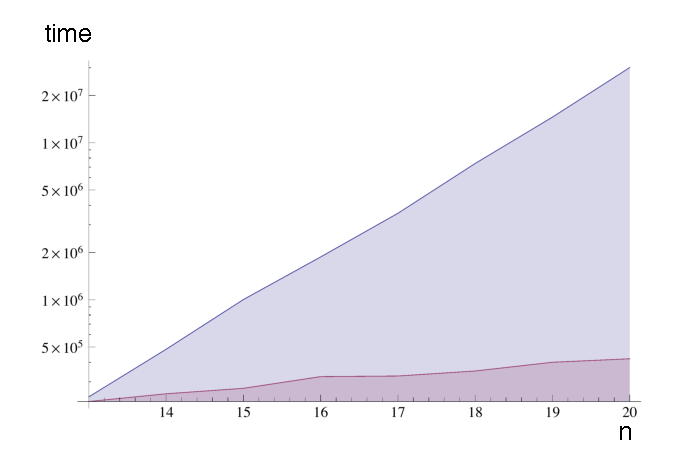
\includegraphics[width=\linewidth]{graphs/pathological-with-axes.pdf}
\caption{\figlabel{patho} Time in nanoseconds for matching $\textit{a?}^n\textit{a}^n$ against input $\textit{a}^n$. Bottom (purple) line is our approach, top (blue) line is java.util.regex.}
\figlabel{patho}
\end{figure}

\begin{table}
\begin{tabular}{ccccccccc|}
\hline 
$n$ & 13 & 14 & 15 & 16 & 17 & 18 & 19 & 20\tabularnewline
\hline 
\hline 
Oracle & 241 & 484 & 1003 & 1874 & 3555 & 7381 & 14561 & 30116\tabularnewline
\hline 
Ours & 225 & 252 & 273 & 32 & 327 & 352 & 400 & 421\tabularnewline
\hline 
\end{tabular}
\caption{Matching times, in microseconds, for matching $\textit{a?}^n\textit{a}^n$ against input $\textit{a}^n$.}
\tablabel{patho}
\end{table}

In the opposite case, in the case of a regular expression that's
crafted to prevent any back-tracking, java.util.regex outperforms
our approach by more than factor 2, as seen in \Tabref{abc} -- but
bear in mind that java.util.regex does not extract parse trees, but
only the last match of all capture groups.  A backtracking
implementation that actually does produce complete parse trees is
JParsec\footnote{\url{http://jparsec.codehaus.org}}, which, as also
seen in \Tabref{abc}, performs on par with our approach, even though
for JParsec never needs to back-track for the input. That may be
because JParsec is a general-purpose parser with much bigger machinery
than java.util.regex, and so, to parse regular expressions, it
follows the same overall algorithm as java.util.regex, but always
with a bigger constant attached.  For this reason, and because
non-greedy matching cannot be expressed directly in JParsec, we did
not implement any further JParsec benchmarks.

\begin{table}
\begin{tabular}{cc}
\hline 
Tool & time\tabularnewline
\hline 
\hline 
JParsec & 4,498\tabularnewline
\hline 
java.util.regex & 1,992\tabularnewline
\hline 
Ours & 5,332\tabularnewline
\hline 
\end{tabular}
\caption{Matching regular expression \texttt{((a+b)+c)+} against input (a\^{}200bc)\^{}2000, where a\^{}200 denotes 200 times character `a'. Time in microseconds.}
\tablabel{abc}
\end{table}

Finally, as a more realistic example, neither chosen to favor
back-tracking nor to avoid it,  extracts all class names, with their
package names, from the project sources itself.  As seen in
\Tabref{real}, our approach outperforms java.util.regex by 40\%,
even though our approach constructs the entire parse tree, and thus
all class names, while java.util.regex outputs only the last matched
class name.

\begin{table}
\begin{tabular}{cc}
\hline 
Tool & time\tabularnewline
\hline 
\hline 
java.util.regex & 11,319\tabularnewline
\hline 
Ours & 8,047\tabularnewline
\hline 
\end{tabular}
\caption{Runtimes, in microseconds, for finding all java class names in all .java files in the project itself. The regular expression used is 
\texttt{(.*?([a-z]+\textbackslash.)*([A-Z][a-zA-Z]*))*.*?}.
Runtime in microseconds}
\tablabel{real}
\end{table}


\section{Related work}
\seclabel{related}
Our algorithm is a modification of Laurikari's algorithm \cite{Laur00a},
which is itself a modified powerset construction algorithm \cite[p. 55]{Sips05a}.

While there is no shortage of books discussing the usage of regular
expressions, the implementation side of regular expression has not
been so lucky. Cox is spot-on when he argues that innovations have
repeatedly been ignored and later reinvented \cite{Cox07a,Cox09a,Cox10a}. 

This paper is no exception. The authors of this paper had set out
to implement Laurikari's TDFA algorithm \cite{Laur00a},
only to discover that Laurikari's description of a TDFA is so far
from complete that it can rightfully only be called the sketch for
an algorithm. Only late in the process did we discover that the blanks
had already been filled by Kuklewicz in the course of his implementation
of TDFAs in Haskell \cite{Kukl07a}. Kuklewicz enshrined his
added insight into Haskell library, but never published the algorithm
as a whole. If the history of regular expressions is evidence of one
thing, it is that source code is a terrible medium to convey algorithms. 

The situation dramatically improved with Cox's simple and concise
explanation of regular expression matching \cite{Cox07a}. It seems
ironic that this well-versed author published this influential work
on his website. The joke, however, may be on Academia's side.

When \del{the taciturn} practioners acknowledge each other's work, we can't
help but disagree almost universally with the characterizations they
produce. Sulzmann and Lu \cite{Sulz12a} call Kuklewicz's
work an ``implementation'' of Laurikari's algorithm, although Laurikari's
algorithm is far too incomplete for that statement to be fair. Laurikari's
algorithm is referred to as a POSIX-style automaton. In truth, Laurikari
leaves the matching strategy entirely open. It was Kuklewicz that
found out how to get POSIX-style matching out of Laurikari's TDFA. 

Cox says that Laurikari's TDFA is a reinvention of \ugh{Pike's published
only in code algorithm} \cite{Pike87a} \on{I can't parse this. Also, there is a publication which is not code, so what do you mean?}, which is Thompson's NFA with
submatch tracking. This seems unfair in that Laurikari's allows for
far more aggressive \chg{reusing}{reuse} of old states than \del{what}
Thompson allows. This should lead to Laurikari's TDFA having fewer
states, and therefore better performance, than even Google's
RE2\footnote{\url{https://code.google.com/p/re2/}}, which uses
Pike's algorithm.  This is not confirmed by the benchmarks by
Sulzmann and Lu \cite{Sulz12a}, but they offer an explanation: in
their profiling, they see that all Haskell implementations spend
considerable time decoding the input strings. In other words, the
measured performance is more of an artifact of the programming
environment used.

Another mistake that permeates the scarce literature is to call regular
expression matching linear. As Sedgewick points out correctly \cite{Sedg90a},
Thompson's NFA matching is of complexity $O(mn)$, where $m$ is the
size of the input NFA, and $n$ is the size of the input string. To
call this linear means to assume that $m$ is fixed, which is not justified. It may well be true that, at present,
$m$ tends to be small. But that is a natural consequence of the algorithms
not scaling very well with $m$. If they did, that would allow for
fast feature extracting from text. Therefore, in this paper, we consider
the state of the art algorithms to be quadratic, since both $m$ and
$n$ are part of the input to a regular expression matcher. We cannot
rule out that a linear algorithm exists, in fact, we hope for it.
To insist that regular expression matching is done in linear time
is to insist that the optimal algorithm has already been found; that
is probably not true.

Sulzmann and Lu add to the table a new matching strategy that yields
good practical performance, although the theoretical bounds are considerably
worse than the state of the art, at $O(n^{2}m)$ \cite{Sulz12a}.

\section{Conclusion}
Our approach can produce entire parse trees while matching regular
expressions.  The performance is on par with traditional back-tracking
solutions if no backtracking ever happens, exponentially outperforms
back-tracking approaches for pathological input, and in a realistic
scenario outperforms backtracking by 40\%.  All source code and all
benchmarks are available under a free license on github.

\bibliographystyle{plain}
\bibliography{biblio,bib/scg}
\end{document}
